
\begin{figure}[H]
  \centering
  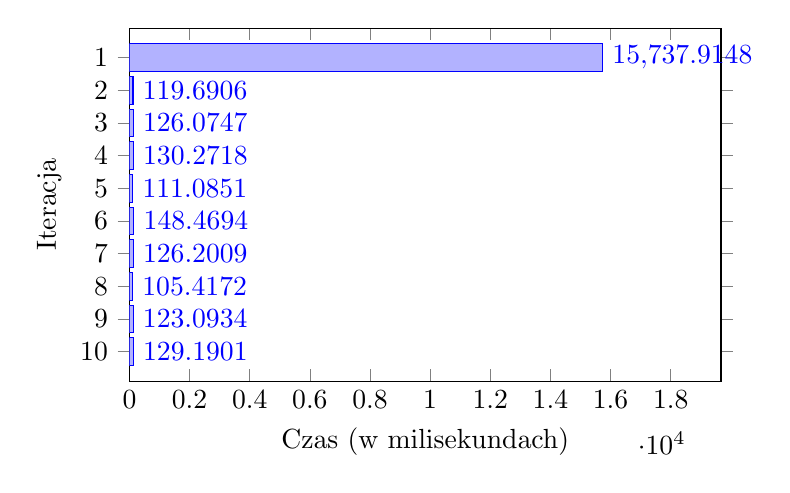
\begin{tikzpicture}
  
    \begin{axis} [
      xbar = .05cm,
      nodes near coords,
      nodes near coords style={
        /pgf/number format/precision=4,
      },
      xmin = 0,
      ytick = data,
      enlarge x limits = {value = .25, upper},
      symbolic y coords = {10,9,8,7,6,5,4,3,2,1},
      xlabel=Czas (w milisekundach),
      ylabel=Iteracja,
      width=0.75\textwidth,
      height=0.5\textwidth
    ]
    
      \addplot coordinates {(15737.91479998827,1) (119.69059997797012,2) (126.07469999790192,3) (130.27179998159409,4) (111.08509999513626,5) (148.46939998865128,6) (126.20090001821518,7) (105.41719996929169,8) (123.09340000152588,9) (129.1900999546051,10)};
      
    \end{axis}
  
  \end{tikzpicture}
  \caption{Wynik testów przykładu 11 [\ref{lst:wydajnosc-przyklad-p-11}]}
  \label{fig:wynik-przyklad-10}
\end{figure}
